% file: graph-decomposition/shortest-cycle-digraph.tex

\documentclass[tikz]{standalone}
\usetikzlibrary{positioning, arrows.meta, chains}

\begin{document}
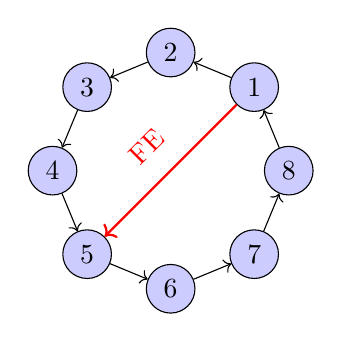
\begin{tikzpicture}[node distance = 1.00cm and 0.10cm, 
      every node/.style = {draw, circle, fill = blue!20},
      every join/.style = {->},
      every edge/.style = {draw, ->},
      start chain = circle placed {at = (\tikzchaincount * 45 : 1.5)}]

      \foreach \i in {1, ..., 8} {
	\node [on chain, join] {\i};
      }

      \draw[->] (circle-end) to (circle-begin);
      \draw[->, red, thick] (circle-1) to node[sloped, above, draw = none, fill = none] {FE} (circle-5);
\end{tikzpicture}
\end{document}
